\section{\normalsize Уравнение Ван-дер-Ваальса как модель неидеального газа. Изотермы газа Ван-дер-Ваальса. Критические параметры. Приведенное уравнение Ван-дер-Ваальса, закон соответственных состояний.}
\paragraph{Уравнение Ван-дер-Ваальса.}
$$\left(P+\dfrac{a\nu^2}{V^2}\right)\left(V-\nu b\right)=RT$$

\begin{wrapfigure}{R}{5cm}
	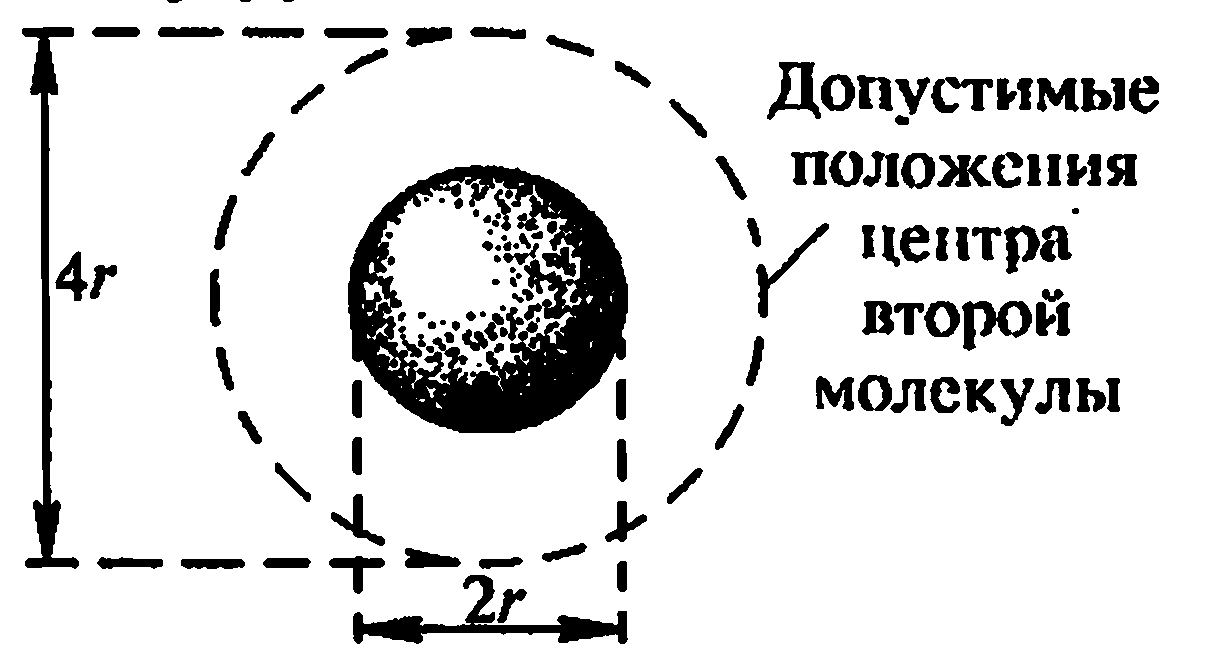
\includegraphics[width=65mm]{ris19.png}
	\caption{Учет конечности размеров молекул}
\end{wrapfigure}
Выведем его, основываясь на $PV=\nu RT$:\\
Во-первых, учтем размеры молекул: \\$\dfrac{4}{3}\pi(2r)^3=8\cdot\dfrac{4}{3}\pi r^3$ --- недоступный объем для второй частицы $\Rightarrow$ в расчете на 1 молекулу $$\dfrac{1}{2}(8\cdot\dfrac{4}{3}\pi r^3)=4V_0$$
где $V_0=4\pi r^3/3$ --- объем одной молекулы. 
В результате объем, разрешенный для движения молекул, cоставит
$$V_\text{доп.} =V-\nu b,\quad$$
$$ b\simeq4\cdot\text{(объем молекулы в одном моле)}=4N_AV_0$$

\begin{wrapfigure}{l}{4cm}
	\label{dipol}
	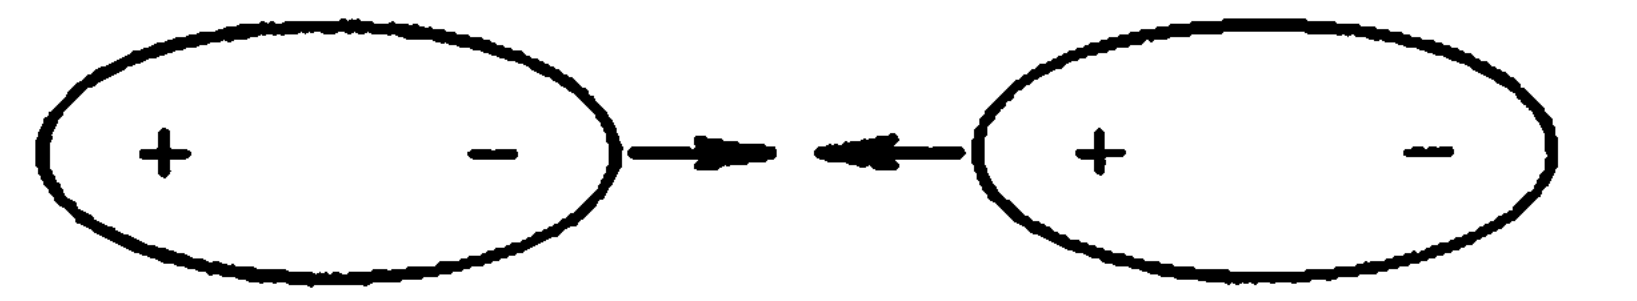
\includegraphics[width=40mm]{ris19_2.png}
	\caption{\small Молекулы--диполи притягиваются друг к другу}
\end{wrapfigure}
Во-вторых, учтем, что молекулы притягиваются друг к другу. Одним из механизмов такого притяжения может быть перераспределение зарядов и образование диполей (см. рис 2).
Давление газа определяется столкновениями молекул со стенкой. Сила, действующая на молекулу у стенки со стороны газа $\sim n$, где $n$ --- число частиц. Частота соударений $\sim n$, значит давление уменьшается на $\Delta P\sim n^2$. Переходя от плотности $n$ к объему $V$ по формуле $n=\dfrac{\nu N_A}{V}$, мы можем записать поправку к давлению в виде $\Delta P=a_1n^2=a(\nu/V)^2.$ Окончательно это дает
$$\left(P+\dfrac{a\nu^2}{V^2}\right)\left(V-\nu b\right)=RT$$
Величины $a$ и $b$ называется параметрами Ван-дер-Ваальса. Параметре $a$ учитывает притяжение, а $b$ --- отталкивание молекул.
\paragraph{Изотермы газа Ван-дер-Ваальса. Критические параметры.}

\begin{wrapfigure}{r}{8cm}
	\label{VdV}
	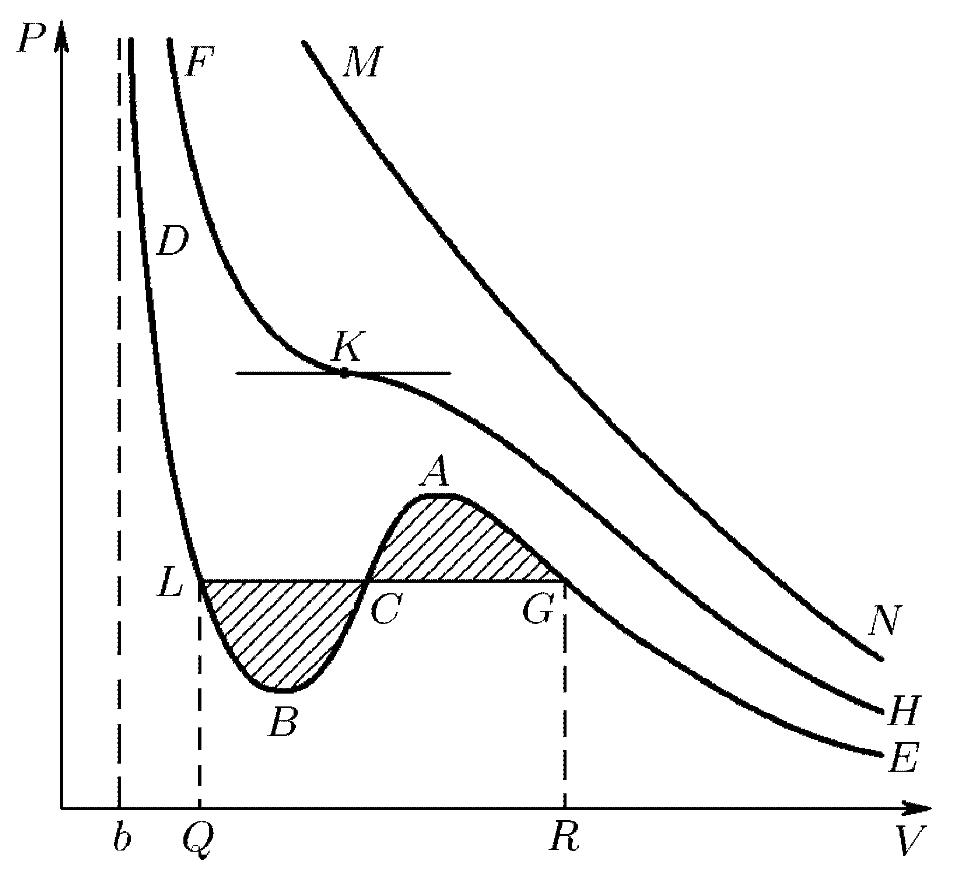
\includegraphics[width=80mm]{ris19_3.png}
	\caption{Изотермы Ван-дер-Ваальса}
\end{wrapfigure}
Уравнение Ван-дер-Ваальса: $$PV^3-(RT+Pb)V^2+aV-ab=0$$ имеет один или три корня. В случае 1 это изотерма MN, а трех --- три пересечения в точках L, C, G изотермы DLBCAGE. При некоторой $T$ $V_1=V_2=V_3$. Такая температура называется \textbf{критической} (изотерма FKH). Для нахождения критических давления, температуры и объема воспользуемся уравнением: $P_\text{к.}~(V~-~V_\text{к.})^3~=~0$\\

\begin{equation*}
\begin{cases}
P_\text{к.}V_\text{к.}^3=ab\\
3P_\text{к.}V_\text{к.}^2=a\\
3P_\text{к.}V_\text{к.}=RT_\text{к.}+P_\text{к.}b
\end{cases}
\Leftrightarrow
\begin{cases}
P_\text{к.}=\dfrac{a}{27b^2}\\
V_\text{к.}=3b\\
T_\text{к.}=\dfrac{8a}{27Rb}
\end{cases}
\end{equation*}
\paragraph{Приведенное уравнение Ван-дер-Ваальса} $\varphi=\dfrac{V}{V_\text{к.}},\quad\pi=\dfrac{P}{P_\text{к.}},\quad\tau=\dfrac{T}{T_\text{к.}}$ --- приведенные параметры. Тогда $V~=~3b\varphi,\quad P~=~\dfrac{a\pi}{27b^2},\\T~=~\dfrac{8a}{27Rb}~\tau\Rightarrow$ \textbf{приведенное уравнение Ван-дер-Ваальса}:
\begin{equation*}
\left(\pi+\dfrac{3}{\varphi^2}\right)(\varphi-1/3)=8/3\tau
\end{equation*}
\paragraph{Закон соответственных состояний.}Уравнение Ван-дер-Ваальса содержит только 3 параметра: $a,\,b,\,R$. Всякое уравнение, обладающее этим свойством, записанное в переменных $\varphi,\,\pi,\,\tau$ должно быть также одинаковым для всех веществ. Это положение есть \textbf{закон соответственных состояний}.\\
\textbf{Соответственными} называют состояния разных веществ, которые имеют одинаковые $\varphi,\,\pi,\,\tau$. Следовательно: если для различных веществ из трех параметров $\varphi,\,\pi,\,\tau$ совпадают значения каких-либо двух, то совпадут и третьи.
